\documentclass[]{article}
\usepackage{lmodern}
\usepackage{amssymb,amsmath}
\usepackage{ifxetex,ifluatex}
\usepackage{fixltx2e} % provides \textsubscript
\ifnum 0\ifxetex 1\fi\ifluatex 1\fi=0 % if pdftex
  \usepackage[T1]{fontenc}
  \usepackage[utf8]{inputenc}
\else % if luatex or xelatex
  \ifxetex
    \usepackage{mathspec}
  \else
    \usepackage{fontspec}
  \fi
  \defaultfontfeatures{Ligatures=TeX,Scale=MatchLowercase}
\fi
% use upquote if available, for straight quotes in verbatim environments
\IfFileExists{upquote.sty}{\usepackage{upquote}}{}
% use microtype if available
\IfFileExists{microtype.sty}{%
\usepackage{microtype}
\UseMicrotypeSet[protrusion]{basicmath} % disable protrusion for tt fonts
}{}
\usepackage[margin=1in]{geometry}
\usepackage{hyperref}
\hypersetup{unicode=true,
            pdftitle={Lecture 6 Homework: Protein Drug Interactions},
            pdfauthor={Corrina Elder},
            pdfborder={0 0 0},
            breaklinks=true}
\urlstyle{same}  % don't use monospace font for urls
\usepackage{color}
\usepackage{fancyvrb}
\newcommand{\VerbBar}{|}
\newcommand{\VERB}{\Verb[commandchars=\\\{\}]}
\DefineVerbatimEnvironment{Highlighting}{Verbatim}{commandchars=\\\{\}}
% Add ',fontsize=\small' for more characters per line
\usepackage{framed}
\definecolor{shadecolor}{RGB}{248,248,248}
\newenvironment{Shaded}{\begin{snugshade}}{\end{snugshade}}
\newcommand{\KeywordTok}[1]{\textcolor[rgb]{0.13,0.29,0.53}{\textbf{#1}}}
\newcommand{\DataTypeTok}[1]{\textcolor[rgb]{0.13,0.29,0.53}{#1}}
\newcommand{\DecValTok}[1]{\textcolor[rgb]{0.00,0.00,0.81}{#1}}
\newcommand{\BaseNTok}[1]{\textcolor[rgb]{0.00,0.00,0.81}{#1}}
\newcommand{\FloatTok}[1]{\textcolor[rgb]{0.00,0.00,0.81}{#1}}
\newcommand{\ConstantTok}[1]{\textcolor[rgb]{0.00,0.00,0.00}{#1}}
\newcommand{\CharTok}[1]{\textcolor[rgb]{0.31,0.60,0.02}{#1}}
\newcommand{\SpecialCharTok}[1]{\textcolor[rgb]{0.00,0.00,0.00}{#1}}
\newcommand{\StringTok}[1]{\textcolor[rgb]{0.31,0.60,0.02}{#1}}
\newcommand{\VerbatimStringTok}[1]{\textcolor[rgb]{0.31,0.60,0.02}{#1}}
\newcommand{\SpecialStringTok}[1]{\textcolor[rgb]{0.31,0.60,0.02}{#1}}
\newcommand{\ImportTok}[1]{#1}
\newcommand{\CommentTok}[1]{\textcolor[rgb]{0.56,0.35,0.01}{\textit{#1}}}
\newcommand{\DocumentationTok}[1]{\textcolor[rgb]{0.56,0.35,0.01}{\textbf{\textit{#1}}}}
\newcommand{\AnnotationTok}[1]{\textcolor[rgb]{0.56,0.35,0.01}{\textbf{\textit{#1}}}}
\newcommand{\CommentVarTok}[1]{\textcolor[rgb]{0.56,0.35,0.01}{\textbf{\textit{#1}}}}
\newcommand{\OtherTok}[1]{\textcolor[rgb]{0.56,0.35,0.01}{#1}}
\newcommand{\FunctionTok}[1]{\textcolor[rgb]{0.00,0.00,0.00}{#1}}
\newcommand{\VariableTok}[1]{\textcolor[rgb]{0.00,0.00,0.00}{#1}}
\newcommand{\ControlFlowTok}[1]{\textcolor[rgb]{0.13,0.29,0.53}{\textbf{#1}}}
\newcommand{\OperatorTok}[1]{\textcolor[rgb]{0.81,0.36,0.00}{\textbf{#1}}}
\newcommand{\BuiltInTok}[1]{#1}
\newcommand{\ExtensionTok}[1]{#1}
\newcommand{\PreprocessorTok}[1]{\textcolor[rgb]{0.56,0.35,0.01}{\textit{#1}}}
\newcommand{\AttributeTok}[1]{\textcolor[rgb]{0.77,0.63,0.00}{#1}}
\newcommand{\RegionMarkerTok}[1]{#1}
\newcommand{\InformationTok}[1]{\textcolor[rgb]{0.56,0.35,0.01}{\textbf{\textit{#1}}}}
\newcommand{\WarningTok}[1]{\textcolor[rgb]{0.56,0.35,0.01}{\textbf{\textit{#1}}}}
\newcommand{\AlertTok}[1]{\textcolor[rgb]{0.94,0.16,0.16}{#1}}
\newcommand{\ErrorTok}[1]{\textcolor[rgb]{0.64,0.00,0.00}{\textbf{#1}}}
\newcommand{\NormalTok}[1]{#1}
\usepackage{graphicx,grffile}
\makeatletter
\def\maxwidth{\ifdim\Gin@nat@width>\linewidth\linewidth\else\Gin@nat@width\fi}
\def\maxheight{\ifdim\Gin@nat@height>\textheight\textheight\else\Gin@nat@height\fi}
\makeatother
% Scale images if necessary, so that they will not overflow the page
% margins by default, and it is still possible to overwrite the defaults
% using explicit options in \includegraphics[width, height, ...]{}
\setkeys{Gin}{width=\maxwidth,height=\maxheight,keepaspectratio}
\IfFileExists{parskip.sty}{%
\usepackage{parskip}
}{% else
\setlength{\parindent}{0pt}
\setlength{\parskip}{6pt plus 2pt minus 1pt}
}
\setlength{\emergencystretch}{3em}  % prevent overfull lines
\providecommand{\tightlist}{%
  \setlength{\itemsep}{0pt}\setlength{\parskip}{0pt}}
\setcounter{secnumdepth}{0}
% Redefines (sub)paragraphs to behave more like sections
\ifx\paragraph\undefined\else
\let\oldparagraph\paragraph
\renewcommand{\paragraph}[1]{\oldparagraph{#1}\mbox{}}
\fi
\ifx\subparagraph\undefined\else
\let\oldsubparagraph\subparagraph
\renewcommand{\subparagraph}[1]{\oldsubparagraph{#1}\mbox{}}
\fi

%%% Use protect on footnotes to avoid problems with footnotes in titles
\let\rmarkdownfootnote\footnote%
\def\footnote{\protect\rmarkdownfootnote}

%%% Change title format to be more compact
\usepackage{titling}

% Create subtitle command for use in maketitle
\newcommand{\subtitle}[1]{
  \posttitle{
    \begin{center}\large#1\end{center}
    }
}

\setlength{\droptitle}{-2em}
  \title{Lecture 6 Homework: Protein Drug Interactions}
  \pretitle{\vspace{\droptitle}\centering\huge}
  \posttitle{\par}
  \author{Corrina Elder}
  \preauthor{\centering\large\emph}
  \postauthor{\par}
  \predate{\centering\large\emph}
  \postdate{\par}
  \date{April 20, 2018}


\begin{document}
\maketitle

\subsection{\texorpdfstring{\emph{Given
Code}}{Given Code}}\label{given-code}

\begin{Shaded}
\begin{Highlighting}[]
\CommentTok{# Can you improve this analysis code?}
\KeywordTok{library}\NormalTok{(bio3d)}
\NormalTok{s1 <-}\StringTok{ }\KeywordTok{read.pdb}\NormalTok{(}\StringTok{"4AKE"}\NormalTok{) }\CommentTok{# kinase with drug}
\end{Highlighting}
\end{Shaded}

\begin{verbatim}
##   Note: Accessing on-line PDB file
\end{verbatim}

\begin{Shaded}
\begin{Highlighting}[]
\NormalTok{s2 <-}\StringTok{ }\KeywordTok{read.pdb}\NormalTok{(}\StringTok{"1AKE"}\NormalTok{) }\CommentTok{# kinase no drug}
\end{Highlighting}
\end{Shaded}

\begin{verbatim}
##   Note: Accessing on-line PDB file
##    PDB has ALT records, taking A only, rm.alt=TRUE
\end{verbatim}

\begin{Shaded}
\begin{Highlighting}[]
\NormalTok{s3 <-}\StringTok{ }\KeywordTok{read.pdb}\NormalTok{(}\StringTok{"1E4Y"}\NormalTok{) }\CommentTok{# kinase with drug}
\end{Highlighting}
\end{Shaded}

\begin{verbatim}
##   Note: Accessing on-line PDB file
\end{verbatim}

\begin{Shaded}
\begin{Highlighting}[]
\NormalTok{s1.chainA <-}\StringTok{ }\KeywordTok{trim.pdb}\NormalTok{(s1, }\DataTypeTok{chain =} \StringTok{"A"}\NormalTok{, }\DataTypeTok{elety =} \StringTok{"CA"}\NormalTok{)}
\NormalTok{s2.chainA <-}\StringTok{ }\KeywordTok{trim.pdb}\NormalTok{(s2, }\DataTypeTok{chain =} \StringTok{"A"}\NormalTok{, }\DataTypeTok{elety =} \StringTok{"CA"}\NormalTok{)}
\NormalTok{s3.chainA <-}\StringTok{ }\KeywordTok{trim.pdb}\NormalTok{(s3, }\DataTypeTok{chain =} \StringTok{"A"}\NormalTok{, }\DataTypeTok{elety =} \StringTok{"CA"}\NormalTok{)}

\NormalTok{s1.b <-}\StringTok{ }\NormalTok{s1.chainA}\OperatorTok{$}\NormalTok{atom}\OperatorTok{$}\NormalTok{b}
\NormalTok{s2.b <-}\StringTok{ }\NormalTok{s2.chainA}\OperatorTok{$}\NormalTok{atom}\OperatorTok{$}\NormalTok{b}
\NormalTok{s3.b <-}\StringTok{ }\NormalTok{s3.chainA}\OperatorTok{$}\NormalTok{atom}\OperatorTok{$}\NormalTok{b}

\KeywordTok{plotb3}\NormalTok{(s1.b, }\DataTypeTok{sse =}\NormalTok{ s1.chainA, }\DataTypeTok{typ =} \StringTok{"l"}\NormalTok{, }\DataTypeTok{ylab =} \StringTok{"Bfactor"}\NormalTok{)}
\end{Highlighting}
\end{Shaded}

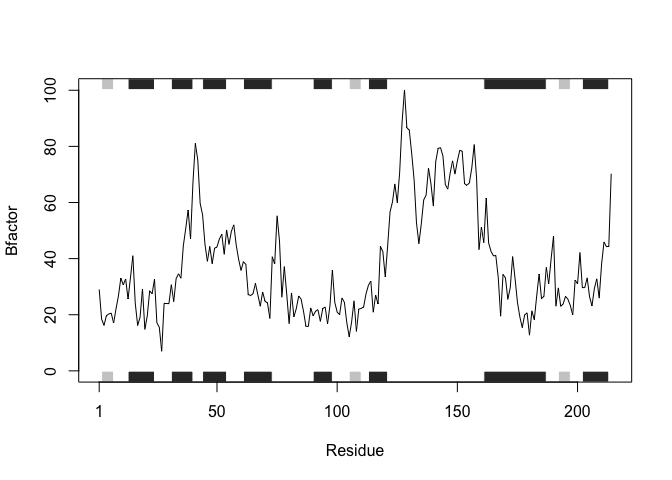
\includegraphics{Lecture_6_Homework_Corrina_Elder_files/figure-latex/unnamed-chunk-1-1.pdf}

\begin{Shaded}
\begin{Highlighting}[]
\KeywordTok{plotb3}\NormalTok{(s2.b, }\DataTypeTok{sse =}\NormalTok{ s2.chainA, }\DataTypeTok{typ =} \StringTok{"l"}\NormalTok{, }\DataTypeTok{ylab =} \StringTok{"Bfactor"}\NormalTok{)}
\end{Highlighting}
\end{Shaded}

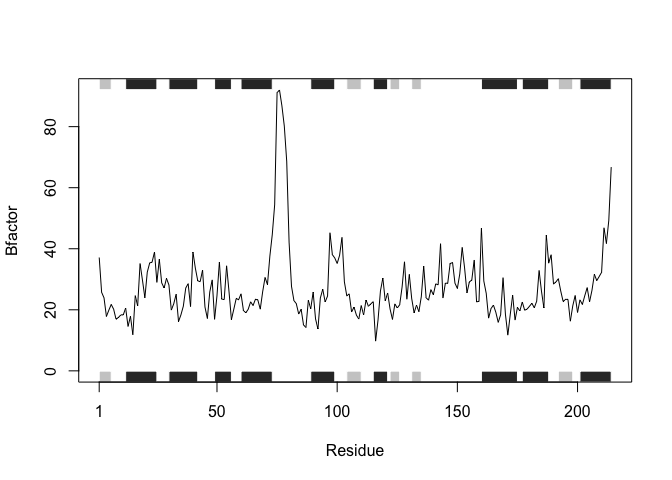
\includegraphics{Lecture_6_Homework_Corrina_Elder_files/figure-latex/unnamed-chunk-1-2.pdf}

\begin{Shaded}
\begin{Highlighting}[]
\KeywordTok{plotb3}\NormalTok{(s3.b, }\DataTypeTok{sse =}\NormalTok{ s3.chainA, }\DataTypeTok{typ =} \StringTok{"l"}\NormalTok{, }\DataTypeTok{ylab =} \StringTok{"Bfactor"}\NormalTok{)}
\end{Highlighting}
\end{Shaded}

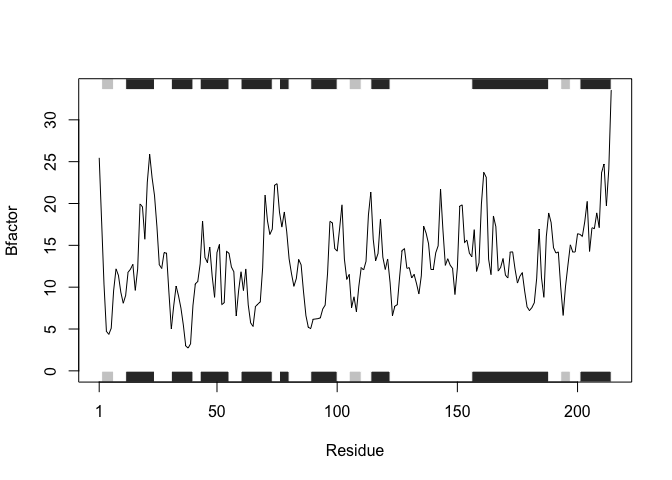
\includegraphics{Lecture_6_Homework_Corrina_Elder_files/figure-latex/unnamed-chunk-1-3.pdf}

\section{\texorpdfstring{\textbf{Q6: How would you generalize the
original code above to work with any set of input protein
structures?}}{Q6: How would you generalize the original code above to work with any set of input protein structures?}}\label{q6-how-would-you-generalize-the-original-code-above-to-work-with-any-set-of-input-protein-structures}

\subsection{What lines of code get repeated for
each?}\label{what-lines-of-code-get-repeated-for-each}

s1 \textless{}- read.pdb(``4AKE'')

s1.chainA \textless{}- trim.pdb(s1, chain = ``A'', elety = ``CA'')

s1.b \textless{}- s1.chainA\(atom\)b s1.chainA\$atom

plotb3(s1.b, sse = s1.chainA, typ = ``l'', ylab = ``Bfactor'')

\subsection{Now to turn this into a
function\ldots{}}\label{now-to-turn-this-into-a-function}

\subsection{\texorpdfstring{This new function,
\textbf{prot\_drug\_plot}, is used to visualize protein drug
interactions from PDB
data.}{This new function, prot\_drug\_plot, is used to visualize protein drug interactions from PDB data.}}\label{this-new-function-prot_drug_plot-is-used-to-visualize-protein-drug-interactions-from-pdb-data.}

\textbf{prot\_drug\_plot} takes in a vector of PDB files as well as
parameters to analyze each file (a chain, an element, and a factor, each
as a string). The function iterates through the files vector, taking the
first item and applying the parameters, then the second, and so on. It
creates the first plot then adds any additional plots to the existing
plot.

The output is one plot (with residues on the x-axis and the specified
factor on the y-axis) with a differently colored line for each file
input.

\emph{The list of colors could be changed/extended to accommodate more
than three unique lines on the plot.}

\begin{Shaded}
\begin{Highlighting}[]
\NormalTok{prot_drug_plot <-}\StringTok{ }\ControlFlowTok{function}\NormalTok{(file, chain, elmnt, fctr) \{}
  
  \CommentTok{# allows our data to be different colors in the graph}
\NormalTok{  plot_colors <-}\StringTok{ }\KeywordTok{c}\NormalTok{(}\StringTok{"cyan"}\NormalTok{, }\StringTok{"orange"}\NormalTok{, }\StringTok{"magenta"}\NormalTok{)}
  
  
  \CommentTok{# to iterate through every value of the file vector}
  \ControlFlowTok{for}\NormalTok{ (i }\ControlFlowTok{in} \DecValTok{1}\OperatorTok{:}\KeywordTok{length}\NormalTok{(file)) \{}
\NormalTok{  s1 <-}\StringTok{ }\KeywordTok{read.pdb}\NormalTok{(file[i])}

\NormalTok{  s1.chain <-}\StringTok{ }\KeywordTok{trim.pdb}\NormalTok{(s1, }\DataTypeTok{chain =}\NormalTok{ chain, }\DataTypeTok{elety =}\NormalTok{ elmnt)}
  
\NormalTok{  atom_df <-}\StringTok{ }\NormalTok{s1.chain}\OperatorTok{$}\NormalTok{atom}
  
  \CommentTok{# the "$" syntax cannot take a variable, so s1.fctr takes in all the atom information and selects an entire column based on the factor input}
\NormalTok{  s1.fctr <-}\StringTok{ }\NormalTok{atom_df[, fctr] }
  
  \CommentTok{# creates the first plot}
  \ControlFlowTok{if}\NormalTok{ (i }\OperatorTok{==}\StringTok{ }\DecValTok{1}\NormalTok{) \{}
    \KeywordTok{plotb3}\NormalTok{(s1.fctr, }\DataTypeTok{sse =}\NormalTok{ s1.chain, }\DataTypeTok{typ =} \StringTok{"l"}\NormalTok{, }\DataTypeTok{ylab =} \KeywordTok{paste}\NormalTok{(}\KeywordTok{toupper}\NormalTok{(fctr), }\StringTok{"factor"}\NormalTok{, }\DataTypeTok{sep =} \StringTok{""}\NormalTok{), }\DataTypeTok{col =}\NormalTok{ plot_colors[i])}
    
    \CommentTok{# adds additional plots to first plot}
\NormalTok{  \} }\ControlFlowTok{else}\NormalTok{ \{}
    \KeywordTok{lines}\NormalTok{(s1.fctr, }\DataTypeTok{col =}\NormalTok{ plot_colors[i])}
\NormalTok{  \}}
\NormalTok{  \}}
  
  \CommentTok{# creates a legend for the graph}
  \KeywordTok{legend}\NormalTok{(}\StringTok{"topright"}\NormalTok{, }\DataTypeTok{title =} \StringTok{"PDB File Name"}\NormalTok{, file, }\DataTypeTok{fill =}\NormalTok{ plot_colors, }\DataTypeTok{horiz=}\OtherTok{TRUE}\NormalTok{, }\DataTypeTok{cex =} \FloatTok{0.5}\NormalTok{, }\DataTypeTok{inset =} \KeywordTok{c}\NormalTok{(}\FloatTok{0.03}\NormalTok{, }\FloatTok{0.06}\NormalTok{))}
\NormalTok{\}}
\end{Highlighting}
\end{Shaded}

\subsection{Test the function with three files and the parameters chain
A, carbon, and factor
b.}\label{test-the-function-with-three-files-and-the-parameters-chain-a-carbon-and-factor-b.}

\begin{Shaded}
\begin{Highlighting}[]
\NormalTok{files <-}\StringTok{ }\KeywordTok{c}\NormalTok{(}\StringTok{"4AKE"}\NormalTok{, }\StringTok{"1AKE"}\NormalTok{, }\StringTok{"1E4Y"}\NormalTok{)}
\NormalTok{chains <-}\StringTok{ "A"}
\NormalTok{elements <-}\StringTok{ "CA"}
\NormalTok{factors <-}\StringTok{ "b"}

\KeywordTok{prot_drug_plot}\NormalTok{(files, chains, elements, factors)}
\end{Highlighting}
\end{Shaded}

\begin{verbatim}
##   Note: Accessing on-line PDB file
\end{verbatim}

\begin{verbatim}
## Warning in get.pdb(file, path = tempdir(), verbose = FALSE): /var/folders/
## fr/kx9dm6l16qz51brxwd8t77b80000gn/T//RtmplfXlsD/4AKE.pdb exists. Skipping
## download
\end{verbatim}

\begin{verbatim}
##   Note: Accessing on-line PDB file
\end{verbatim}

\begin{verbatim}
## Warning in get.pdb(file, path = tempdir(), verbose = FALSE): /var/folders/
## fr/kx9dm6l16qz51brxwd8t77b80000gn/T//RtmplfXlsD/1AKE.pdb exists. Skipping
## download
\end{verbatim}

\begin{verbatim}
##    PDB has ALT records, taking A only, rm.alt=TRUE
##   Note: Accessing on-line PDB file
\end{verbatim}

\begin{verbatim}
## Warning in get.pdb(file, path = tempdir(), verbose = FALSE): /var/folders/
## fr/kx9dm6l16qz51brxwd8t77b80000gn/T//RtmplfXlsD/1E4Y.pdb exists. Skipping
## download
\end{verbatim}

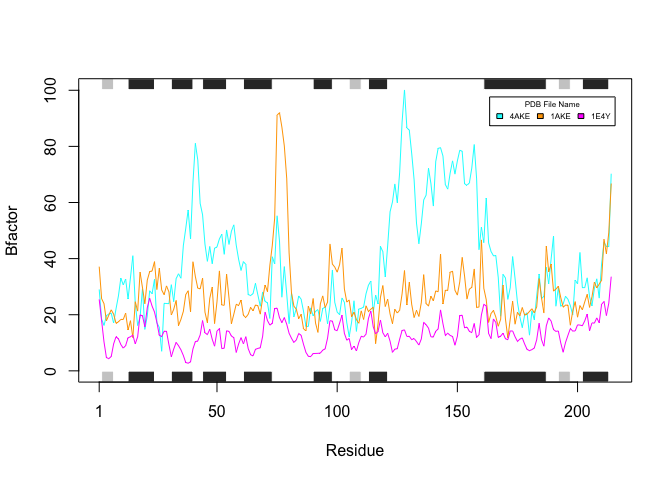
\includegraphics{Lecture_6_Homework_Corrina_Elder_files/figure-latex/unnamed-chunk-3-1.pdf}


\end{document}
